\documentclass[10pt,a4paper]{article}
\usepackage[top=1in, bottom=1.25in, left=1in, right=1in]{geometry}

\usepackage[T1]{fontenc}
\usepackage{amsmath}
\usepackage[utf8]{inputenc}
\usepackage{polski}
\usepackage{graphicx}
\usepackage{float}
\usepackage{amssymb}
\usepackage{amsthm}
\usepackage{hyperref}
\usepackage {tikz}
\usetikzlibrary {positioning}
%\usepackage {xcolor}
\definecolor {processblue}{cmyk}{0.96,0,0,0}

\title{\vspace{-2cm}Obrona - przygotowanie}
\begin{document}
  \maketitle
%http://www.mimuw.edu.pl/~son/ML/ML2016/

% \section{Algorytmy aproksymacyjne 1: algorytmy kombinatoryczne}
% \paragraph{2-aproksymacyjny dla problemu minimalnego pokrycia wierzchołkowego}
% Około 20. minuty: \url{http://was.zaa.mimuw.edu.pl/?q=node/38}
% \begin{figure}[H]
%   \centering
%     \includegraphics[scale=0.50]{images/amazonOpinia.png}
%   \caption{Przykładowe wypowiedzi użytkowników pobrane z portalu \textit{Amazon}}
% \end{figure}
\section{Uczenie maszynowe}
\subsection{Support Vector Machine}
  \begin{itemize}
    \item classification, regression; classification - find hyper-plane that differentiate the two classes very well
    \item maximizing the distances between nearest data point and hyper-plane (distance - Margin); low margin - high chance of mis-classification
    \item kernel (allows the algorithm to fit the maximum-margin hyperplane in a transformed feature space)- function which takes low dimensional input space and transform it ingo a higher dimensional space; used in non-linear separation problems; examples: polynomial, gaussian
    \item hyperplane: largest separation, magrin : distance from hyperplane to the nearest data point on each size is maximized (maximum-margin hyperplane)
  \end{itemize}
Margines klasyfikatora liniowego: szerokość bezpiecznego obszaru po obu stronach hiperpłaszczyzny; margines wyznaczony jest przez 2 hiperpłaszczyzny, szukamy klasyfikatora z maksymalnym marginesem.
\begin{figure}[H]
  \centering
    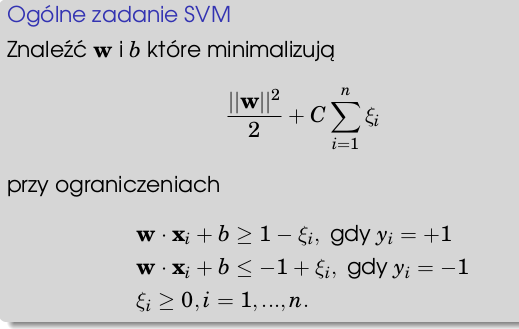
\includegraphics[scale=0.50]{images/zadSVM.png}
\end{figure}
\begin{figure}[H]
  \centering
    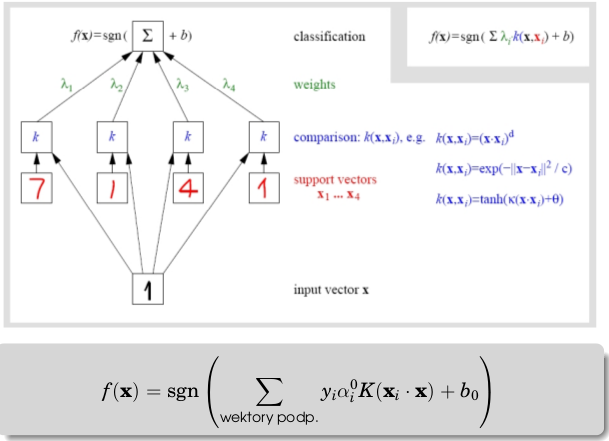
\includegraphics[scale=0.50]{images/svm2.png}
\end{figure}
\subsection{Latent Semantic Analysis}
  \begin{itemize}
    \item analyzing relationships between a set of documents and the terms they contain by \textbf{producing set of concepts related to the documents and terms}
    \item Assumption: words that are close in meaning will occur in similar pieces of text
    \item Singular value decomposition (SVD) - used to reduce number of rows while preserving structure among columns; $X = U \Sigma V^{T}$, $U, V$ - orthogonal matrices ($Q^{T} = Q^{-1}$), $\Sigma$ - diagonal matrix; values on diagonal $\Sigma$ - singular values; application: given a query of terms, translate it into the low-dimensional space and find matching documents.
    \begin{figure}[H]
      \centering
        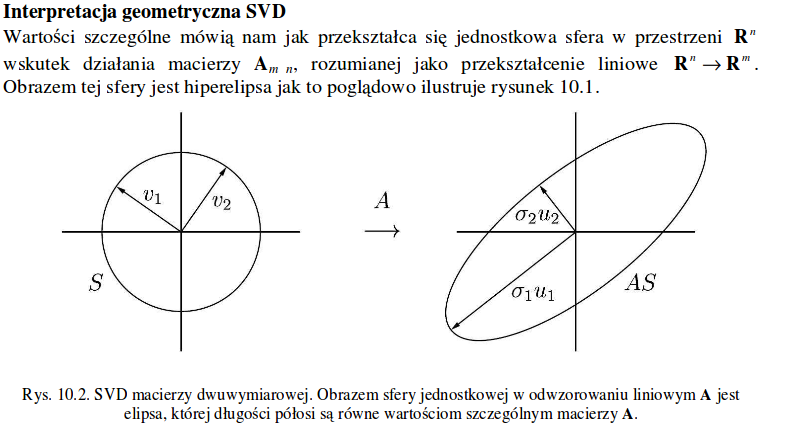
\includegraphics[scale=0.50]{images/svd.png}
    \end{figure}
    \item LSA limitations: results difficult to interpret, cannot capture multiple meanings of a words,
    \item Latent Semantic Indexing (LSI) - ability to extract the conceptual content of a body of text by establishing associations between those terms that occur in similar contexts

  \end{itemize}
\subsection{Ocena klasyfikatorów}
  \begin{itemize}
    \item Minimalizujemy $FP+FN$, procedura, zbiory: treningowe, walidacyjne (optymalizacja parametrów), testowe
    \item Walidacja krzyżowa, testowanie każdego podzbioru używając pozostałych jako zbiór treningowy, błedy wszystkich iteracji są uśredniane, aby otrzymać błąd globalny; \textbf{walidacja pozwala na zmiejszenie długości przedziału ufności}
    \item kroswalidacja stratyfikowana - podział obiektów pomiędzy zbiór treningowy i testowy, aby zostały zachowane oryginalne proporcje pomiędzy klasami decyzyjnymi; ważne - gdy w zbiorze danych występują znaczne dysproporcje w liczebności przykładów do poszczególnych klas decyzyjnych
    \item leave-one-out - dla n obiektów budujemy klasyfikator n razy
    \item bootstrap - szacowanie rozkładu błedów estymacji za pomocą wielokrotnego losowania ze zwracaniem z próby
    \item miary: sensitivity (TPR) $TPR = TP/(TP+FN)$ : RECALL
    \item krzywa LIFT - obrazuje zysk z zastosowania modelu klasyfikacyjnego względem nie stosowania modelu; $CPH(p)$ - (Cumulative Percentage Hit) część klasy docelowej znajdująca się wśród $p\%$ pierwszych obiektów z listy rankingowej
    \item True positive rate (trafienie) $TPR(p) = TP / (TP + FN)$; odsetek fałszywych alarmów $FPR(p) = FP / (FP+TN)$
  \end{itemize}
\begin{figure}[H]
  \centering
    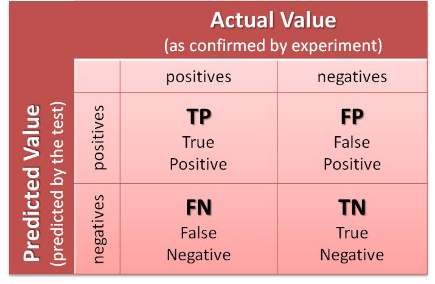
\includegraphics[scale=0.50]{images/macierz.png}
\end{figure}
\subsection{Drzewo decyzyjne}
\begin{itemize}
  \item węzły: testy na wartościach atrybutów; liście - decyzje o klasyfikacji obiektów
  \item funkcje testów: operujące na pojedynczych atrybutach, testy będące kombinacją wartości kilku atrybutów
  \item dla większości parametrów, problem szukania optymalnego drzewa jest NP-trudny
  \item kryterium stopu: zbiór obiektów pusty, obiekty z jednej klasy decyzyjnej, brak podziału przez żaden test; etykiety wyznaczone zasadą większościową
  \item miary róźnorodności zbioru: conflict, entropia : przyjmują największą wartość, gdy rozkład klas decyzyjnych w zbiorze X jest równomierny; najmniejszą wartość - gdy wszystkie obiekty w X są jednej kategorii
  \item miary do oceny testów: \textit{liczba par obiektów rozróżnianych przez test } (liczymy na podstawie conflict) lub \textit{kryterium przyrostu informacji} - liczymy na podstawie entropii; własności: monotoniczność, funkcje ocen testu przyjmują małe wartości jeśli rozkłady decyzyjne w podzbiorach są zbliżone
  \item ocena funkcji testu: rozróżnialność, przyrost informacji, wspólczynnik przyrostu informacji
\end{itemize}
\subsection{Sieci neuronowe}
Zbiór połączonych ze sobą jednostek wejściowo-wyjściowych, z każdym połączeniem skojarzona jest waga, która może zostać zmieniona w trakcie uczenia.
\begin{figure}[H]
  \centering
    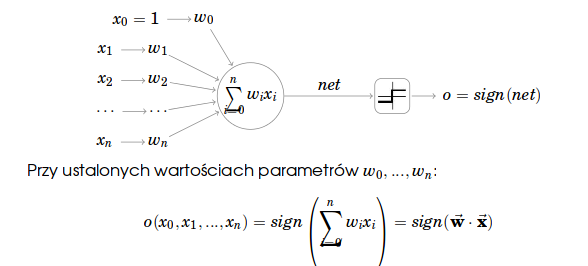
\includegraphics[scale=0.50]{images/siec.png}
\end{figure}
Ważne: sieć może nauczyć się przewidywania sygnałów wyjściowych bez jawnego zdefiniowania związku między danymi wejściowymi a wyjściowymi.
\begin{figure}[H]
  \centering
    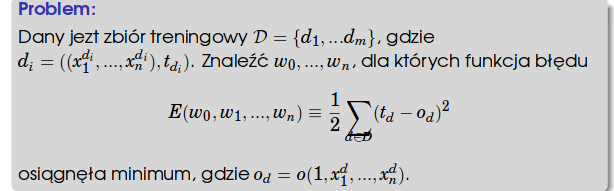
\includegraphics[scale=0.50]{images/perc.png}
\end{figure}
\begin{itemize}
  \item nieliniowe perceptrony: nieliniowe, ciągłe i różniczkowalne funkcje aktywacji nauronów  np. logistyczna funkcja sigmoidalna, tangens hiperboliczny...
  \item architektura sieci: liczba ukrytych warstw, liczba neuronów w każdej warstwie, funkcja aktywacji, współczynnik uczenia się, kodowanie danych wejściowych i wyjściowych, warunek stopu i problem przeuczenia się; wiedza w sieciach przechowywana jest w wagach połączenia między neuronami
\end{itemize}
\paragraph{Self-organizing map}: artificial neural network that is trained using unsupervised learning to produce a low-dimensional, discretized representation of the input space of the training samples; sieć neuronowa Kohonena; zalety: może rozpoznawać skupienia występujące w danych wejściowych oraz kojarzyć podobne klasy, umożliwia lepsze zrozumienie danych; np. sieć dostarcza topologicznego odwzorowania z przestrzeni wielowymiarowej na dwuwymiarową mapę jednostek, zachowuje nieliniowe relacje między jednostkami i umieszcza bliskie sobie jednostki w pobliżu siebie na mapie; struktura:
\begin{figure}[H]
  \centering
    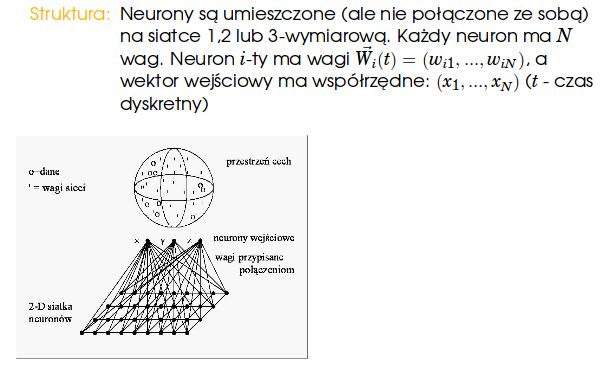
\includegraphics[scale=0.50]{images/som.png}
\end{figure}

\subsection{Metody selekcji istotnych cech i ekstrakcji nowych}
Zadanie: znaleźć minimalny zbiór atrybutów, który zachowuje najistotniejsze charakterystyki zbioru wszystkich atrybutów. \\
Heurystyczne metody selekcji:
  \begin{itemize}
    \item selekcja pojedynczych dobrych cech za pomocą testów istotności przy założeniu o niezależności cech
    \item selekcja lokalnie najlepszych w każdym kroku
    \item eliminacja pojedynczych cech
    \item metoda optymalnego podziału i ograniczeń
  \end{itemize}
Redukcja wymiarowości:
  \begin{itemize}
    \item \textbf{PCA: Principal component analysis} - znajdujemy kierunki, które zachowują największą wariancję danych; używana do zmiejszania rozmiaru danych statystycznych poprzez odrzucenie ostatnich czynników; celem PCA jest taki obrót układu współrzędnych, aby zmaksymalizować w pierwszej kolejności wariancję pierwszej współrzędnej a następnie wariancję drugiej współrzędnej; zawężenie wymiaru przestrzeni - z otrzymanych wartości własnych wybieramy te największe - celem minimalizacji straty informacji podczas rzutowania danych na miejszą liczbę wymiarów. Procedura: wybór zmiennych do analizy, wyznaczenie macierzy korelacji, wyznaczenie głownych składowych, rotacja głównych składowych, interpretacja
    \item \textbf{SVD: Singular value decomposition}
    \item supervised and nonlinear techniques
  \end{itemize}
  Metody klasyfikacji: testy statystyczne, użycie funkcji entropii, Gini index (miara nierówności rozkładu zmiennej losowej)
\subsection{Wnioskowanie Boolowskie w obliczaniu reduktów i reguł decyzyjnych}
%WAZNE: http://www.mimuw.edu.pl/~son/ML/ML2016/W6.pdf
Wnioskowanie Boolowskie:
  \begin{enumerate}
    \item Modelowanie: kodowanie problemu za pomocą układu równań
    \item Redukcja: sprowadzenie układu równań do pojedynczego równania
    \item Konstrukcja: znalezienie wszystkich implikantów pierwszych funkcji
    \item Dedukcja: zastosowanie pewniej sekwencji wnioskowań transformujących implikanty pierwsze do rozwiązań problemu
  \end{enumerate}
  \paragraph{Szukanie reduktów} : usuwanie alternatyw regułą pochłaniania
  \begin{figure}[H]
    \centering
      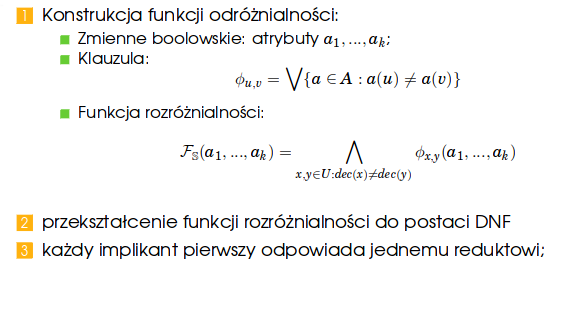
\includegraphics[scale=0.50]{images/redukt.png}
  \end{figure}
  \paragraph{Heurystyka Johnsona} : algorytm zachłanny
  \begin{enumerate}
      \item Znaleźć atrybut, który występuje najczęściej w macierzy rozróżnialności
      \item usunąć wszystkie pola zawierające wybrany atrybut
      \item powtórzyć 1, 2 dopóki wszystkie pola macierzy są puste.
  \end{enumerate}
  Heurystyki: Integer Linear Program, Symulowane wyżarzanie, algorytmy genetyczne
  \paragraph{Systemy decyzyjne oparte o zbiory przybliżone} :
  \begin{figure}[H]
    \centering
      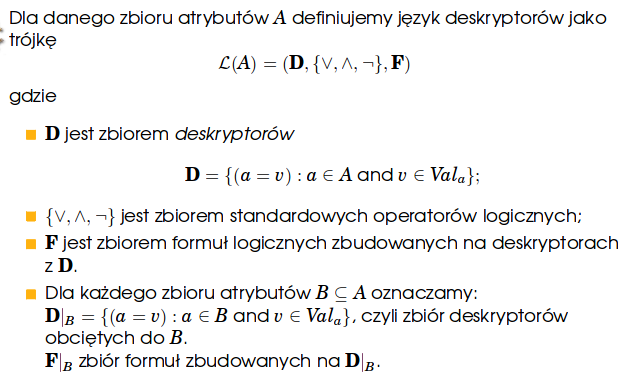
\includegraphics[scale=0.50]{images/des.png}
  \end{figure}
  \begin{figure}[H]
    \centering
      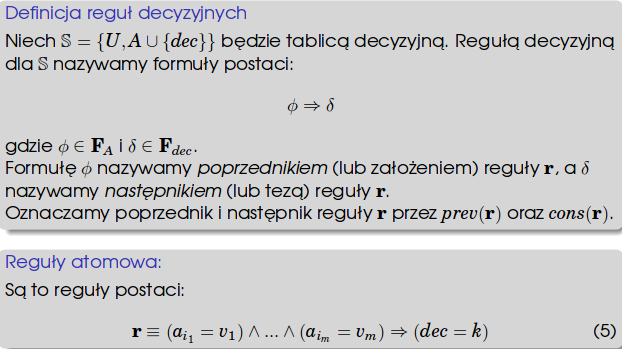
\includegraphics[scale=0.50]{images/regula.png}
  \end{figure}
  Charakterystyka reguł: liczba deskryptorów występujących w założeniu reguły, nośnik reguły: zbiór obiektów spełniających założenie reguły; support - liczba obiektów spełniających założenie reguły; confidence: wiarygodność reguły \\
  Metody odkrywania reguł z danych: metoda sekwencyjnego pokrycia- reguły sekwencyjnie wyszukiwane dla każdej klasy decyzyjnej; \textbf{metoda oparta o drzewo decyzyjne}: każda ścieżka od korzenia do liścia definiuje jedną regułę, generuje zbiór reguł, które tworzą rozłączne pokrycie zbioru obiektów
  \subsection{Wymiar Wapnika-Czerwonienkisa}
  Stanowi miarę mocy wyrażania pojęć danej przestrzeni hipotez, definiowany jest jako liczność największego zioru, który jest rozbijany przez przestrzeń hipotez. \\
  Shattering: \\
  \begin{figure}[H]
    \centering
      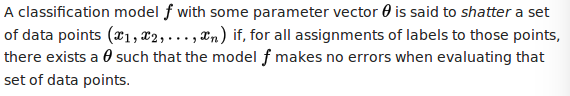
\includegraphics[scale=0.50]{images/shatter.png}
  \end{figure}
  Definition: The VC dimension of model f is the maximum number of points that can be arranged so that f shetters them. It is a maximum integer D s.t. some data point set of cardinality D can be shattered by f.
  \begin{figure}[H]
    \centering
      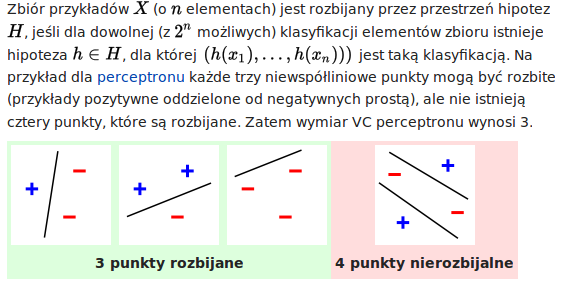
\includegraphics[scale=0.50]{images/rozbijanie.png}
  \end{figure}
  Fundamentalne twierdzenia: \\
  Warunek konieczny: jeśli przestrzeń hipotez ma nieskończony wymiar VCdim to nie jest potencjalnie wyuczalna. \\
  Fundamentalne: Jeśli przestrzeń hipotez ma skończony wymiar VC, to jest potencjalnie wyuczalna.

\subsection{Clustering}
Uczenie bez nadzoru, a klasyfikacja to metoda przewidywania przynależności obiektów do klas decyzyjnych. \\
Dane: liczba klastrów, funkcja odległości określona na zbiorze obiektów, funkcja oceny jakości klastrów; Problem: podział zbioru obiektów na k klastrów, tak aby funkcja jakości przyjmowała maksymalną wartość
  \begin{itemize}
    \item k-means: struktura płaska, określone deterministycznie
    \begin{figure}[H]
      \centering
        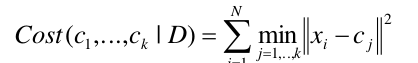
\includegraphics[scale=0.50]{images/koszt.png}
    \end{figure}
    Nowy centroid jest środkiem cięzkości powstającego w poprzednim przebiegu algorytmu, klastra. Jakoś klastrów zależą od wyboru początkowego układu centroidów, alg. może trafić w lokalne minimum.
    \item grupowanie hierarchiczne: struktura drzewiasta, określone deterministycznie - budowanie drzewa klastrów dla zioru obiektów; najniższy poziom n liści, każdy jest klastrem; repeat: znajdź najbliższą parę klastrów (parę poddrzew) i je połącz \\
    Odległości między klastrami: single linkage, complete linkage, ...
    \item probabilistyczne grupowanie: struktura płaska klastrów, określone probabilistycznie: obiekt należy do klastra z pewnym stopniem prawdopodobieństwa, każdy klaster jest opisany jednym rozkładem prawdopodobieństwa; założenie: wszystkie rozkłady są rozkładami normalnymi różniącymi się wartościami oczekiwanymi i odchyleniami standardowymi
  \end{itemize}
  Miary odległości: Euclidean, Hamming, Minkowski, ..\\
  Zastosowanie: kwantyzacja wektorowa, redukcja obrazów \\
  Twierdzenie: problem grupowania minimalnego względem sumy kwadratów błędów jest NP-trudny nawet dla $k = 2$. \\
  Wybór liczby grup - analiza zmiany funkcji jakości klastrów w zależności od liczby klastrów. \\
  \textbf{Algorytm EM} (Expection - Maximization): dana liczba klastrów k, dla każdego atrybutu rzeczywistego znależć k układów parametrów (opisy klastrów) : wartość oczekiwana, odchylenie standardowe, ....,
  \begin{figure}[H]
    \centering
      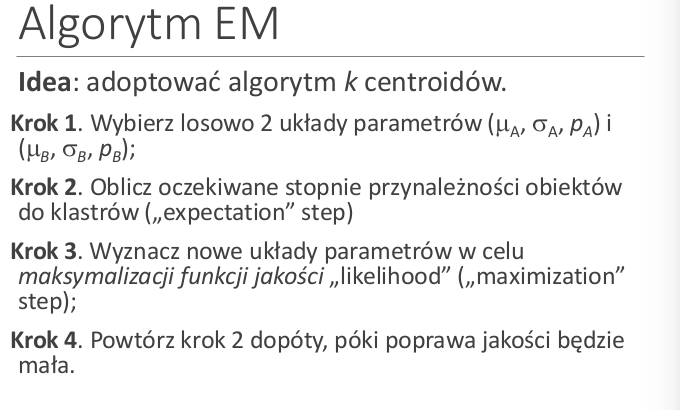
\includegraphics[scale=0.50]{images/algEM.png}
  \end{figure}
\subsection{Hidden Markov Model}

\subsection{Sieci rekurencyjne}
W sieciach rekurencyjnych istnieją \textbf{sprzężenia zwrotne między wejściem, a wyjściem}.
  \begin{itemize}
    \item Dla ustalonej architektury sieci i konfiguracji parametrów, znalezienie optymalnego układu wag jest co najmniej NP-trudne.
    \item predykcja: na podstawie danych wejściowych przewidywać dane wyjściowe, bez konieczności definiowania związku między danymi wejściowymi a wyjściowymi; klasyfikacja i rozpoznawanie; \textbf{kojarzenie i analiza danych}: wykrywanie istotnych powiązań między danymi
  \end{itemize}
\textbf{Sieć Hopfielda}: %TODO przygotowac opis; dopracować sieci rekurencyjne
\subsection{Boosting. Metoda wzmocnienia klasyfikatorów}
%TODO: doczytac z innych materialow
Idea: budowanie mocnego i złożonego klasyfikatora ze słabych i prostych klasyfikatorów. \\
\textbf{AdaBoost} (Adaptive Boosting) - wywołuje wybrany słaby algorytm uczący w serii T iteracji. \textbf{Główna idea}: utrzymywanie rozkładu wag dla zbioru treningowego.
\begin{itemize}
  \item Po każdej iteracji wagi źle sklasyfikowanych elementów są zwiększane (skierowanie uwagi na słaby klasyfikator).
  \item Zadaniem słabego algorytmu uczącego jest zbudowanie klasyfikatowa dla aktualnego rozkładu wag.
  \item Skuteczność klasyfikatora jest mierzona przez jego błąd z uwzględnieniem rozkładu wag z danej iteracji.
  \item Kiedy AdaBoost dostaje klasyfikator dobierany jest parametr $\alpha$, który odpowiada za wagę jaką przykładamy do tego klasyfikatora.
  \item Rozkład wag zmieniany tak, aby zwiększyć (zmniejszyć) wagi elementów zbioru treningowego, które są źle klasyfikowane. \\
\end{itemize}
Pseudokod algorytmu:
\begin{figure}[H]
  \centering
    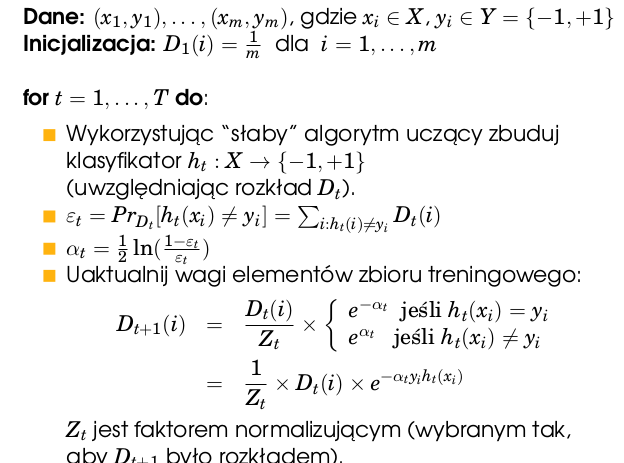
\includegraphics[scale=0.50]{images/pseudo.png}
\end{figure}
Wynikowy klasyfikator:
\begin{figure}[H]
  \centering
    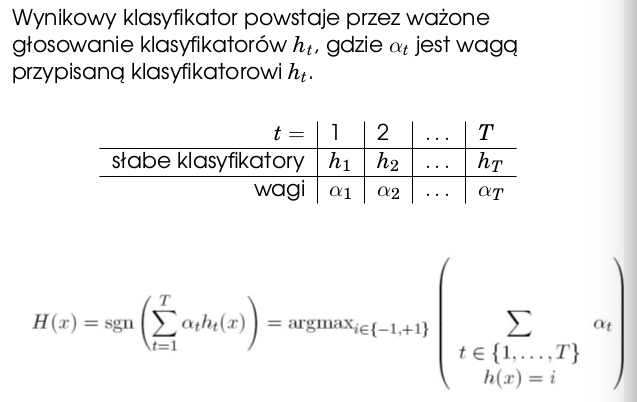
\includegraphics[scale=0.50]{images/wynik.png}
\end{figure}
Własności algorytmu AdaBoost:
\begin{itemize}
  \item zdolność do zredukowania błędu na zbiorze treningowym.
  \item oszacowanie ogólnego błędu wynikowego klasyfikatora z wykorzystaniem: błędu na zbiorze treningowym $m$, wymiaru Vapnika $d$ dla klasy słabych klasyfikatorów (mierzy umiejętność algorytmów klasyfikacji - największa liczba punktów jakie algorytm może rozbić w dowolny sposób) oraz ilości iteracji algorytmu wzmacniania $T$.
  \begin{figure}[H]
    \centering
      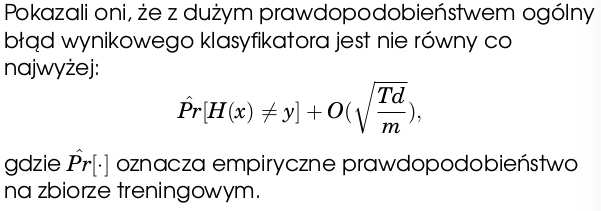
\includegraphics[scale=0.50]{images/praw.png}
  \end{figure}
  \item zdolność do wykrywania przypadków nietypowych poprzez zwiększanie wag elementów źle sklasyfikowanych
  \item wrażliwy na szumy w danych
\end{itemize}
\section{Data mining}
\subsection{Transaction data analysis and association rules}
Sample rule : $X$ and $Y$; result $Z$
  \begin{itemize}
    \item support - probability that a transaction contains $X, Y, Z$
    \item confidence - conditional probability that a transaction having $X, Y$ also contains $Z$ (support($X$ and $Y$)$/$ support($Z$))
  \end{itemize}
Mining Association Rules: generate all frequent itemsets; generate high confidence association rules from each frequent itemset \\
\textbf{Apriori principle}: if an itemset is frequent then all of its subsets must also be frequent. Observation: if an itemset is infrequent, then all of its supersets must also be infrequent. \\
\textbf{Algorithm}: \textit{bottom up approach}, frequent subsets are extended one item at a time and groups of candidates are tested against the data. \\
\begin{itemize}
    \item count support of candidates itemsets are stored in a hash-tree
\end{itemize}
\textbf{Rule generation}: given a frequent itemset $L$, find all non-empty subsets $f$ of itemset s.t. $f -> L$ - $f$ satisfies the minimum confidence requirement.
\section{Rough Sets}
\section{Matematyczne pojęcia}
\paragraph{Statystyka} : %TODO pomóc Tomkowi
\paragraph{Chi-square} : any statistical hypothesis test wherein the sampling distribution of the test statistic is a chi-square distribution when the null hypothesis is true. Example: test - that variance of a normally distributed population has a given value based on a sample variance. \\
\paragraph{Wartość własna} :
  \begin{figure}[H]
    \centering
      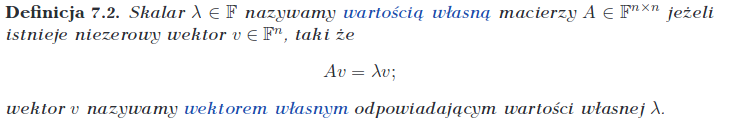
\includegraphics[scale=0.50]{images/wartosc.png}
  \end{figure}
  \begin{figure}[H]
    \centering
      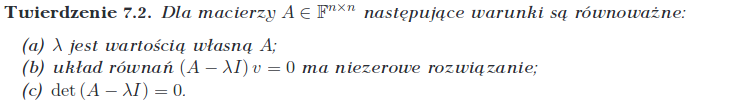
\includegraphics[scale=0.50]{images/wartosc2.png}
  \end{figure}
\paragraph{Macierz kowariancji} :
\begin{figure}[H]
  \centering
    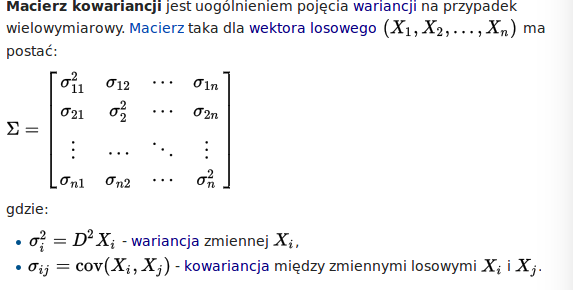
\includegraphics[scale=0.50]{images/cov.png}
\end{figure}
\paragraph{Postać DNF} : formuła jest w postaci DNF, jeśli jest ona alternatywą klauzul, z których każda jest koniunkcją literałów.
\end{document}
